
\chapter[AM generation and Demodulation using AD 633]{AM generation and Demodulation using AD 633}
\section*{Aim}
To design and implement AM generation and demodulation using multiplier IC AD633.
\section*{Theory}
DSB-SC using AD633 has already been discussed in chapter \ref{chapdsbsc}. DSB-SC is same as AM devoid of the carrier. Inorder to obtain the pure AM waveform which is \emph{double side band with carrier}, add the carrier signal to the DSB-SC signal.
\paragraph{}
	The resultant AM can be demodulated in two ways,
 \begin{enumerate}
\item
Using another AD633 in cascade with AM generating circuit.
\item
Using Diode envelope detector.

\end{enumerate}
\section*{Design}
Provide the biasing voltage of +15 V to pin 8 of the IC and -15 V to pin 5 of the IC.\\

To the \textbf{X} and \textbf{Z} inputs of the IC, feed the carrier sinusoid of amplitude $E_m=2.5\ V$ and frequency $f_m= 1\ kHz$.\\
To the \textbf{Y} input of the IC, feed the message sinusoid of amplitude $E_c=2.5\ V$ and frequency $f_c= 10\ kHz$.\\

The output AM signal will have a waveform as given by,

\begin{equation}
W=\frac{X.Y}{10}+Z
\end{equation}
\begin{equation}
W=\frac{e_m.e_c}{10}+e_c
\end{equation}
\begin{equation}
W=\frac{6.25}{20}[cos 2\pi 9t-cos 2\pi 11t]+2.5 sin(2\pi10t)
\end{equation}

Thus it contains two sidebands and the carrier.

\section*{Circuit Diagram}
\section*{Procedure}
\section*{Observation}
The input and output signals as observed on a CRO are shown in Figure \ref{AM633plot1}and \ref{AM633plot2}.
\begin{figure}
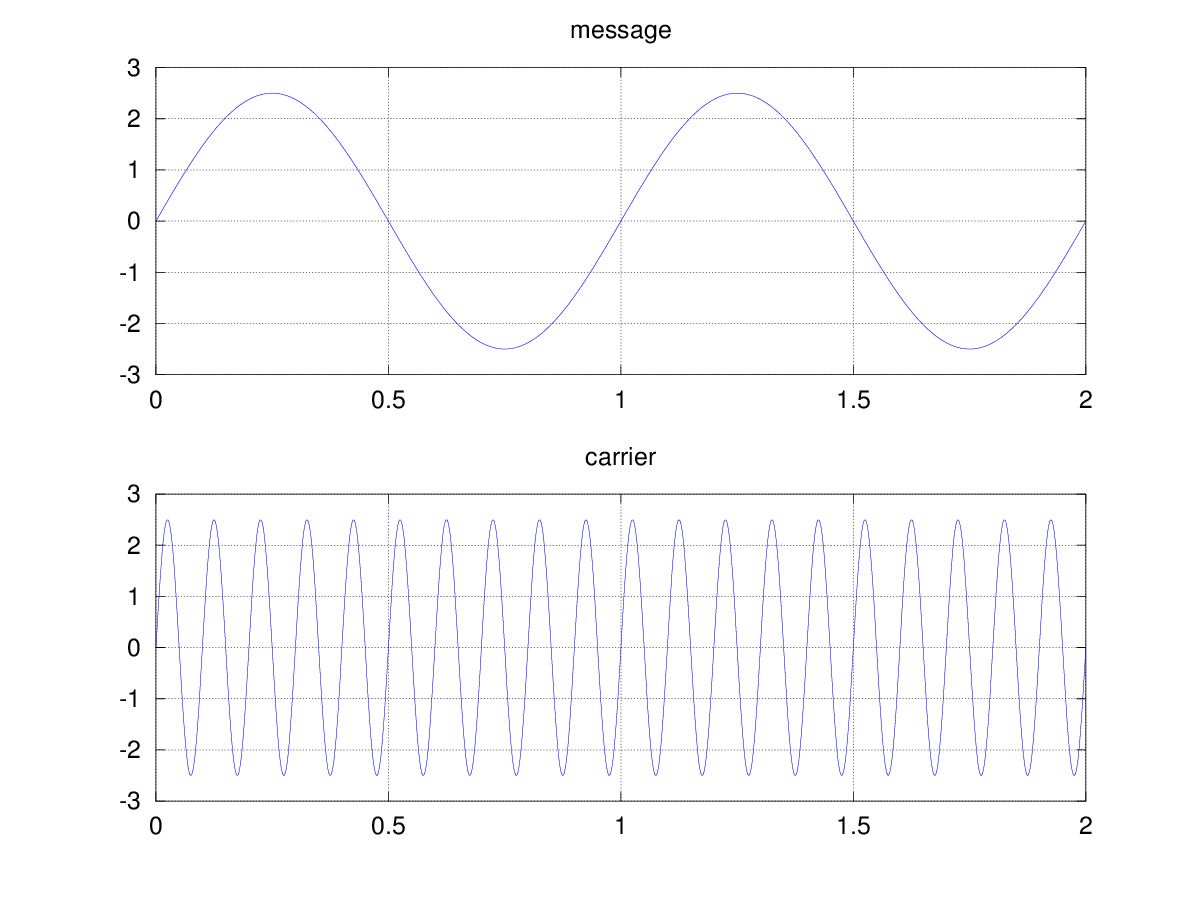
\includegraphics[width=\textwidth]{am6331.png}
\caption{Message and carrier signals}
\label{AM633plot1}
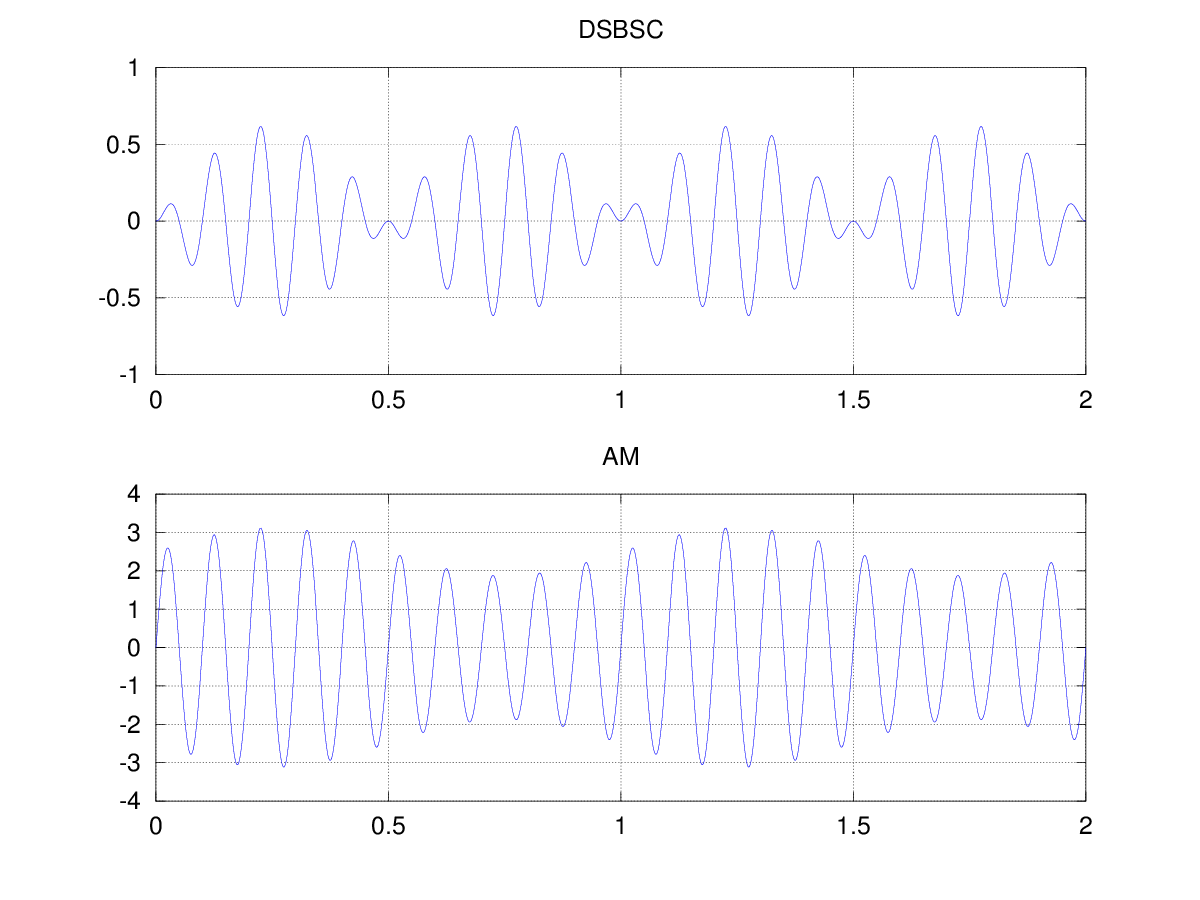
\includegraphics[width=\textwidth]{am6332.png}
\caption{DSBSC and AM signals}
\label{AM633plot2}
\end{figure}


\section*{Result}